\documentclass[11pt]{article}
\usepackage{amsmath,amssymb} 
\usepackage{geometry}
\usepackage{graphicx}
\usepackage{float}
\usepackage{flafter}
\usepackage{subcaption}
\geometry{a4paper,scale=0.72}

\author{Weihao Jiang, 519021911045}
\title{Report: Weighted Round-Robin
scheduler}
\date{\today} 

\begin{document}
\maketitle

\section{Introduction}\label{introduction}

CPU scheduling is the basis of multiprogrammed operating systems. By
switching the CPU among processes, the operating system can make the
computer more productive. The Linux
kernel, and the Android OS built on top of it, uses both
First-in-First-out (\textbf{FIFO}) queuing and round robin (\textbf{RR})
strategies to build its real-time tasks scheduler, and the completely
fair scheduling (\textbf{CFS}) algorithm to build its default task
scheduler. We implement here a weighted round robin (\textbf{WRR})
scheduler and compare the typical features of different schedulers.

As in the original requirement, our implementation of the WRR scheduler
sets the scheduling weights and time slices only according to whether it
is a foreground or a background application. However, the distinction
does not bring out the true power of the WRR scheduler, so we modified
it by making a system call that allows the task weights to be modified,
and demonstrated this in the scheduler comparison.

We also implemented several utilities to help us inspect and change
scheduling policies. To provide an image of the comparison between
schedulers, we have also written a process testing tool.

\section{Analysis and
Implementation}\label{analysis-and-implementation}

\subsection{\texttt{wrr.c}, the scheduler}\label{wrrc-the-scheduler}

In order to design our scheduler, we first studied the scheduler
mechanism of linux. We found that linux uses the \texttt{sched\_class}
structure to implement the scheduler in order to abstract different
scheduling mechanism. Therefore, our scheduler implementation is mainly
to implement the \texttt{sched\_class} structure of the \texttt{WRR}
scheduler, which is mainly in \texttt{kernel/sched/wrr.c}. To provide
better structured information, we have also added a header file
\texttt{kernel/sched/wrr.h} that is only referenced in \texttt{wrr.c}.

In the requirements, we do not need to implement SMP, i.e. the symmetric
multiprocessor architecture, so we ignore all SMP-related contents when
implementing. In addition, our WRR here is more oriented to scheduling
common tasks than RT scheduler scheduling real-time tasks, and in the
requirements we also set the weights through the task group mechanism,
so instead of using the task group and group inheritance scheduling
structure like the real-time tasks, we use an overall round robin
mechanism, and each polling will be selected among all tasks that use
the WRR scheduling mechanism.

Our WRR structure here requires the use of task groups to distinguish
between the foreground and background. Therefore, we refer to the
relevant function \texttt{task\_group\_path()} in the \texttt{debug.c}
file to get the task group name and thus determine the foreground and
background. In this implementation, the weight is updated every time it
happens to enqueue or dequeue, and when the time slice is being
refreshed.

The main implementation of the rest of the content refers to the
original real-time scheduler section. However, we do not need the part
of the real-time scheduler about priority, so instead of using a bitmap
structure, we operate directly on a list. This (list) operation process
is also reflected in the real-time scheduler, because in fact the
real-time scheduler also contains the round robin scheduling algorithm.

\subsection{Embedding into the
system}\label{embedding-into-the-system}

In order to add our WRR scheduler to the kernel, we need to make some
adjustments to the original system content.

\begin{itemize}
\item
  Compile Flags

  We introduced a new compile flag \texttt{CONFIG\_WRR\_GROUP\_SCHED},
  which will automatically generated into a header file at compile time
  and define this macro. Add this
  option to the \texttt{init/Kconfig} file and add
  \texttt{CONFIG\_WRR\_GROUP\_SCHED=y} to the
  \texttt{arch/arm/configs/goldfish\_armv7\_defconfig} file so that this
  macro is defined.

  We have introduced a number of debugging statements at the time of
  coding and they are all defined under the
  \texttt{CONFIG\_SCHED\_DEBUG} macro. However, these printing
  operations cause a lot of extra overhead for the scheduler, so we
  created a new file
  \texttt{arch/arm/configs/goldfish\_armv7\_nodebug\_defconfig} here to
  disable it and save the overhead. The \texttt{task\_group\_path()}
  mentioned above also needs to be adjusted at this point, as removing
  this macro will make a function from \texttt{autogroup.h} invalid.
\item
  Linux header files

  We adjusted \texttt{include/linux/sched.h} to define the
  \texttt{SCHED\_WRR} macro identifier and some values for weights and
  time slices. We declared \texttt{wrr\_rq} as \texttt{rt\_rq} do.

  we also defined \texttt{sched\_wrr\_entity} structure to store
  necessary information for each WRR task: a link\_head
  \texttt{run\_list} for WRR task queueing, \texttt{time\_slice} and
  \texttt{weight} for weighting and time slice counting. After defining
  we added an instance \texttt{wrr} into \texttt{task\_struct}.
\item
  Scheduler Makefile

  Added \texttt{wrr.o} to link our \texttt{wrr.c} into the scheduler.
\item
  Scheduler \texttt{rt.c}

  Set the next scheduler of the RT scheduler to be the WRR scheduler
  (originally it would be the CFS scheduler), so that the main scheduler
  will be scheduled in the order RT - WRR - CFS.
\item
  Scheduler \texttt{core.c}

  Added the time slice update and weight update related operation
  functions for WRR. Since other schedulers do not set the weights in
  WRR, we need this function to set them when switching schedulers.

  We initialize lists of WRR, allowable values, etc., just like the RT
  do. \texttt{core.c} has a common judgment: if it is a real-time task,
  set it to \texttt{rt\_sched\_class}, otherwise set it to
  \texttt{fair\_sched\_class}. We use the \texttt{policy} value of the
  task to determine this and set the task with the WRR policy to
  \texttt{wrr\_sched\_class}.

  We refine the judgment of the value of \texttt{policy} in the related
  function of the task scheduler switching.
\item
  Scheduler \texttt{sched.h}

  defined struct \texttt{wrr\_rq}, which is the running queue of WRR.
  the list\_head \texttt{active} points to the head of the queue of
  \texttt{sched\_wrr\_entity}, and \texttt{wrr\_nr\_running} indicates
  the running task number in the WRR queue.
\end{itemize}

\subsection{Testing utilities}\label{testing-utilities}

In order to test the scheduler more easily, we wrote two utilities
\texttt{lshed} and \texttt{chshed}. By using the system calls
\texttt{sched\_setscheduler} and \texttt{sched\_rr\_get\_interval}, the
former can output the used scheduler and time slice information based on
the input PID, and the latter can change the scheduler and scheduling
parameters for a specific PID.

Since the given \texttt{processtest.apk} is not very comprehensive in
what it tests, we also wrote a \texttt{proctest} test program that forks
a specified number of test processes and specifies their schedulers and
scheduling parameters. The test process simulates a common CPU burst /
IO burst loop, waiting for a certain number of seconds (simulates an IO
waiting) after a large number of adding loop (which is a CPU burst), and
print out the loop time.

\section{Test Results}\label{test-results}

Here we test with the provided file \texttt{processtest.apk}. In fig.\ref{fig:switch} we use the
utility \texttt{lshed} and \texttt{chshed} mentioned above to manipulate
the scheduler.
\begin{figure}[H]
  \centering
  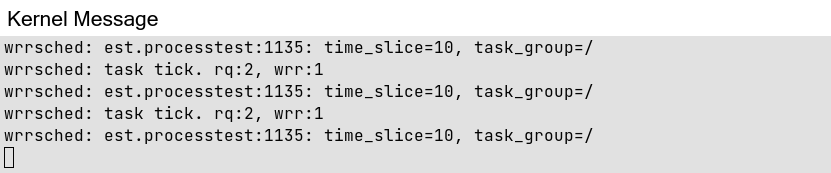
\includegraphics[width=0.8\textwidth]{.split/change-sched.1.png}
  \phantomcaption
\end{figure}
\begin{figure}[H]\ContinuedFloat
  \centering
  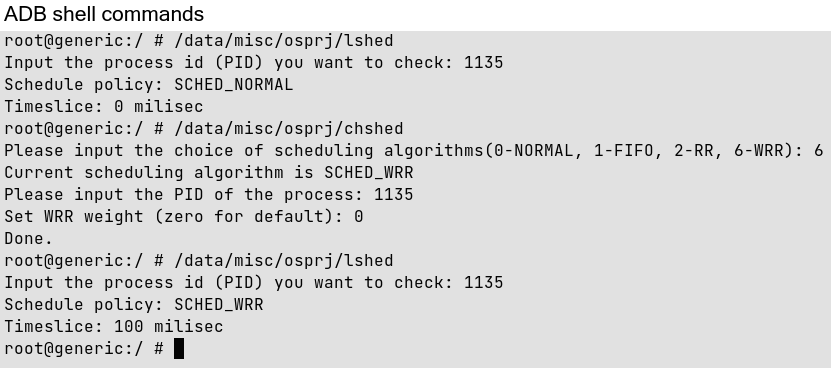
\includegraphics[width=0.8\textwidth]{.split/change-sched.2.png}
  \caption{switch the scheduler}\label{fig:switch}%
\end{figure}


Here in fig.\ref{fig:fg2bg} we changed the \texttt{processtest} application from foreground to
background, by clicking the home button, and here are the results. We
may read from \texttt{lshed} result that the new time slice is set to 10
ms. We may see from the figure below that in some rounds the time\_slice
did not decrease. This is because the time slice is refreshed when the
task is rejoined. Here, because the program performs a short refresh
action, it does not use up a tick (10ms) before re-entering the wait
state and exiting the queue. A more complete scheduling process can be
observed in the fig.\ref{fig:bg2fg}.

\begin{figure}[H]
\centering
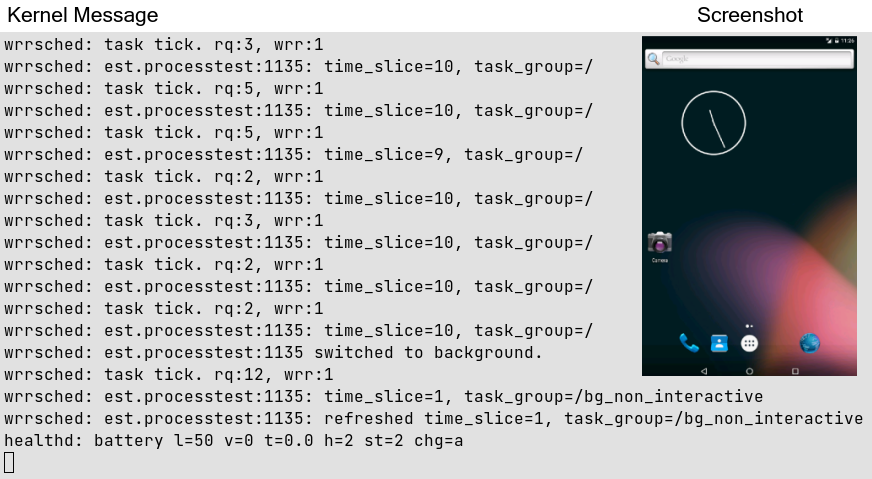
\includegraphics[width=0.8\textwidth]{.split/fg-to-bg.1.png}
\phantomcaption
\end{figure}
\begin{figure}[H]\ContinuedFloat
  \centering
  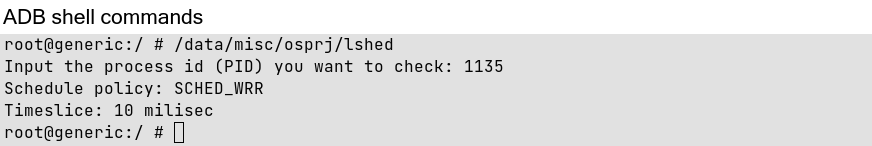
\includegraphics[width=0.8\textwidth]{.split/fg-to-bg.2.png}
  \caption{change the \texttt{processtest} application from foreground to
  background}
  \label{fig:fg2bg}
  \end{figure}

When we switched from background to foreground by android
application switcher, you may see that in fig.\ref{fig:bg2fg}
the time\_slice is updated to 10,
which indicates 100 ms, as 10 ms for a time tick.

\begin{figure}[htb!]
\centering
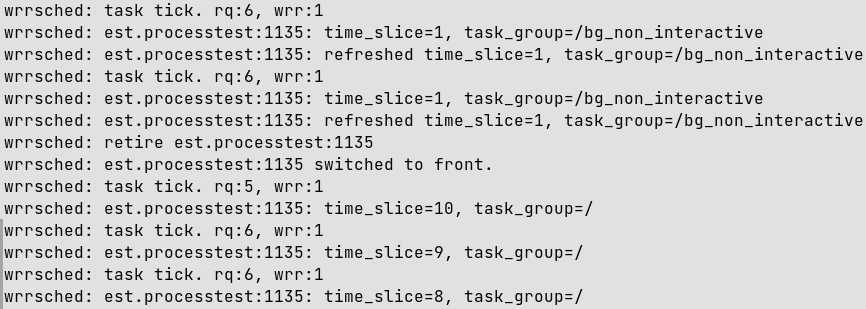
\includegraphics[width=0.75\textwidth]{bg-to-fg.png}
\caption{change the \texttt{processtest} application from background to
foreground}
\label{fig:bg2fg}
\end{figure}

\section{Additional Part}\label{additional-part}

\subsection{Throttle Mechanism}\label{throttle-mechanism}

Because the main scheduler is scheduled sequentially, i.e. the later
scheduler will be called only when the previous one has finished
scheduling. Therefore, when intensive tasks are executed with WRR
policy, it will be difficult for the CFS scheduler immediately after it
to get time for running. Since the vast majority of the system's tasks,
including \texttt{adb}, display, and control, are executed under the CFS
scheduler, this will make the entire virtual machine not responding.

Following the example of the throttle mechanism in the real-time
scheduler, we have introduced this mechanism in the WRR scheduler to
share more runtime with other schedulers (i.e. CFS scheduler).

\subsection{Adjustable Weight}\label{adjustable-weight}

There are many programs, especially those executing on the linux level
(the other example is the android level), that do not use task groups to
distinguish themselves. For example, the android debug bridge, and all
programs forked from the adb shell, behave as so-called foreground
programs. This degrades the WRR scheduler to a normal RR scheduler in
most situations.

Therefore we modified the implementation functions behind the
\texttt{sched\_setscheduler} and \texttt{sched\_setparam} system calls,
and also modified \texttt{sched\_wrr\_entity} appropriately to enable
flexible adjustment of the weights. Since the \texttt{sched\_param}
structure is defined in the GNU C library and not in the kernel, it is
difficult to adjust the contents of this structure, so we have reused
the priority in the configuration real-time task. Setting this value to
a non-negative value manually adjusts the weight of the task, while
setting it to 0 restores the original weighting convention.

This feature is critical to utilize the WRR scheduler's full ability,
and is applied in the comparison of scheduler features that follows.

\subsection{Scheduler Comparison}


We now compare the scheduler implemented in Linux with the scheduler we
wrote to analyze their typical features and similarities. Linux
scheduler seems to have a wide range of six scheduling strategies, but
in fact there are only three: FIFO scheduling, RR scheduling and CFS
scheduling (although Deadline scheduling was introduced later in the
Linux kernel, the 3.4.67 kernel used in the experiment does not have
this scheduling method). Here we discuss the performance of each
scheduler with the same priority (or weight) and with different
priorities (or weights). 

\emph{Since the priority of CFS is more complex
and not directly related to the set value, we will only discuss the
performance of CFS under the same priority.}

\subsubsection{Scheduling with the same priority}

The conclusions for RR scheduling and FIFO scheduling, when the
priorities are the same, are trivial. Because the same policy is used,
these scheduling methods are consistent with the result that each
process has the same weight in WRR scheduling. Unlike CFS scheduling,
which executes out-of-order because of using the red-black tree as
organizational structure, these scheduling algorithms remains a good
sequential order. The main difference is performance.

Our test program is set to 10 processes, and for WRR scheduling the
weight is set to the default weight of the foreground program (i.e. 100
ms, the same as RR scheduling).

\begin{table}[H]
  \centering
  \begin{tabular}{r|cccc}
    \hline
Scheduler & FIFO & RR & CFS & WRR \\
Approx. Time & 250 ms & 2000 ms & 2500/4500 ms & 4500 ms \\\hline
\end{tabular}
\end{table}

Because of the different scheduling algorithms adopted and the different
priorities (meaning the priority of the scheduler), in fig.\ref{fig:fifosame} 
we observe that the
FIFO scheduler takes the shortest time per loop. Once the FIFO scheduler
is running it is not preempted by programs of the same or lower
priority, and we can interpret this value as the time to run centrally.

\begin{figure}[ht]
  \begin{subfigure}{.5\textwidth}
    \centering
    % include first image
    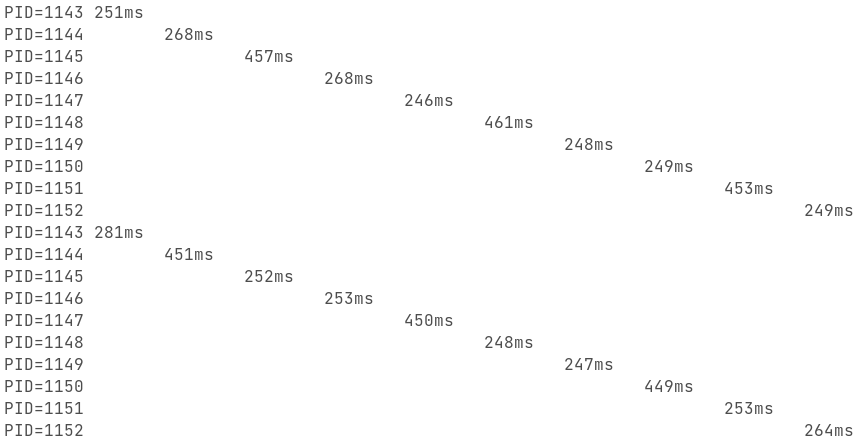
\includegraphics[width=\textwidth]{FIFO-example.png}
    \caption{FIFO scheduling, same priority}
    \label{fig:fifosame}
  \end{subfigure}
  \begin{subfigure}{.5\textwidth}
    \centering
    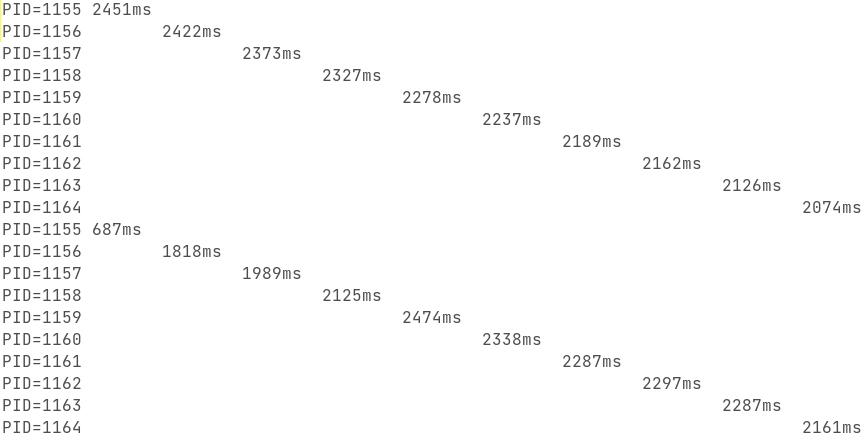
\includegraphics[width=\textwidth]{RR-step-example.png}
    \caption{RR scheduling, same priority}
    \label{fig:rrsame}
  \end{subfigure}
  \newline
  \begin{subfigure}{.5\textwidth}
    \centering
    % include first image
    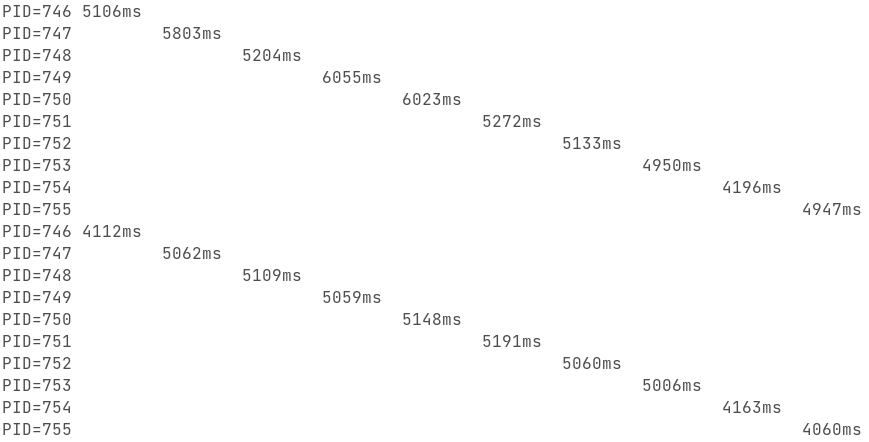
\includegraphics[width=\textwidth]{WRR-sameW-example.png}
    \caption{WRR scheduling, same weight}
    \label{fig:wrrsame}
  \end{subfigure}
  \begin{subfigure}{.5\textwidth}
    \centering
    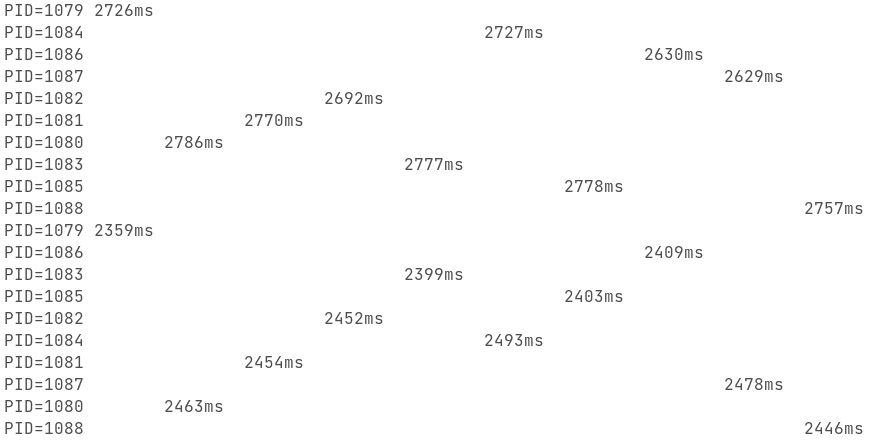
\includegraphics[width=\textwidth]{CFS-example.png}
    \caption{CFS scheduling, same nice value}
    \label{fig:cfssame}
  \end{subfigure}
  \caption{Same priority scheduling}
  \label{fig:same}
  \end{figure}


We may see that in fig.\ref{fig:rrsame} 
the time of the RR scheduler grows significantly, but it actually meets
our expectation. 100 ms is the length of the RR time slice, which means
that the previous 250 ms will be divided into three time slice
executions. The average time taken by the RR scheduler is around 2000
ms, which is as expected.


For WRR scheduling shown in fig.\ref{fig:wrrsame}, because of the throttle mechanism implemented in the
previous section, WRR scheduling leaves 50\% of the time for the CFS
scheduler. Coupled with the fact that WRR scheduling runs after
real-time tasks with lower priority, such time spent is reasonable.


We can observe that the in fig.\ref{fig:cfssame} time variance for CFS is smaller and it
completes faster (about 2500 ms). (This is because the WRR scheduler is
in idle state. When we fill up the WRR scheduler, the CFS scheduler takes
a similar amount of time as the WRR scheduler, but the time gap is still
smaller than the WRR scheduler.) The CFS scheduler, as the default
scheduler for Linux, shows its advantages of stability and efficiency.

\subsubsection{Scheduling with different priorities}

It is easy to know that FIFO scheduling at different priority levels
tends to cause starvation of lower priority programs. But the RR
scheduling used in real-time scheduling does not bring any improvement
either, because the low-priority programs in the real-time scheduler do
not run while the high-priority programs is running (That's why the
real-time task scheduler provides throttling to reserve some runtime to
the waiting successor scheduler and the low-priority processes). 
As fig.\ref{fig:rtdiff} shows, FIFO
scheduling and RR scheduling performed in the same behavior. Thus both
exhibit low priority processes being starved to death. We see that the
process in seventh place of the priority list takes a minute to complete
a cycle, and the three processes further down have never output from the
start.

\begin{figure}[ht]
  \begin{subfigure}{.5\textwidth}
    \centering
    % include first image
    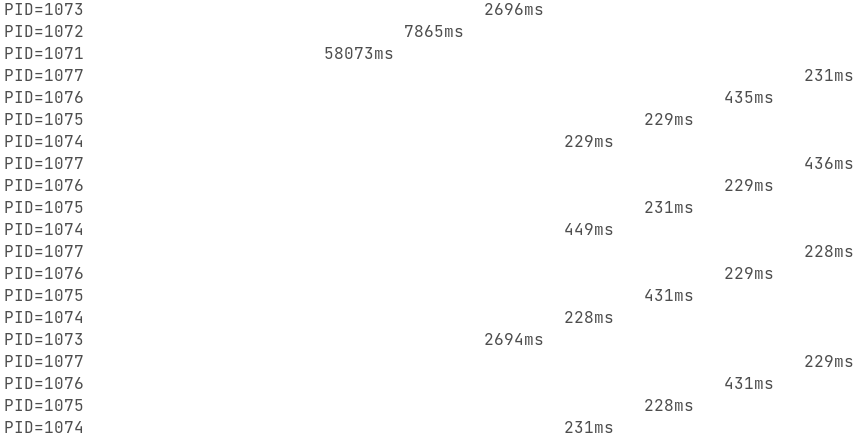
\includegraphics[width=\textwidth]{RT-example.png}
    \caption{RR/FIFO scheduling, different priorities}
    \label{fig:rtdiff}
  \end{subfigure}
  \begin{subfigure}{.5\textwidth}
    \centering
    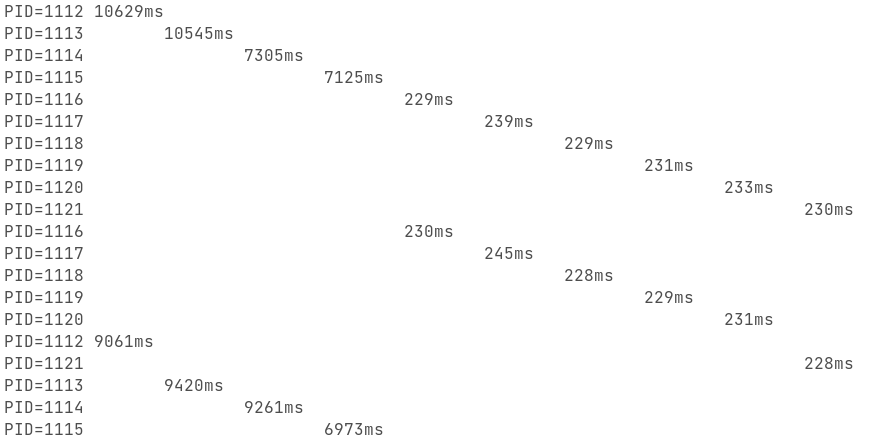
\includegraphics[width=\textwidth]{WRR-example.png}
    \caption{WRR scheduling, different weight}
    \label{fig:wrrdiff}
  \end{subfigure}
  \caption{Differnt priorities scheduling}
  \label{fig:diff}
  \end{figure}

Our WRR scheduler then shows the advantage of starvation-free. And
because the time slice setting is increased, more processes are able to
run undisturbed (with similar performance to FIFO scheduling in same
priority scheduling), and the lower priority processes do not wait too
long. We see from fig.\ref{fig:wrrdiff} the process at the beginning of the line (i.e. the one with the
shortest time slice) has a time slice of only 150 ms, but still manages
to finish in about ten seconds. There is no starvation of the program.
This is determined by the stack characteristics of WRR.

\section{Conclusion}\label{conclusion}

Through this project, I have gained a deeper understanding of the
scheduler in the linux kernel. By combining kernel-level programming
with application-level programming, I gradually understood their
similarities and differences. It was especially gratifying to see that
my additions to the kernel could be performed and called correctly by
the outer programs. From understanding the implementation of a large
project, to editing, compiling and debugging it, them all forms a great
challenge which could not be found in past practical courses, and I
think this project is very practical and instructive for future
programming practice.

\end{document}
